\section{Physics improvements for photon interactions}

\begin{figure}
	\centering
    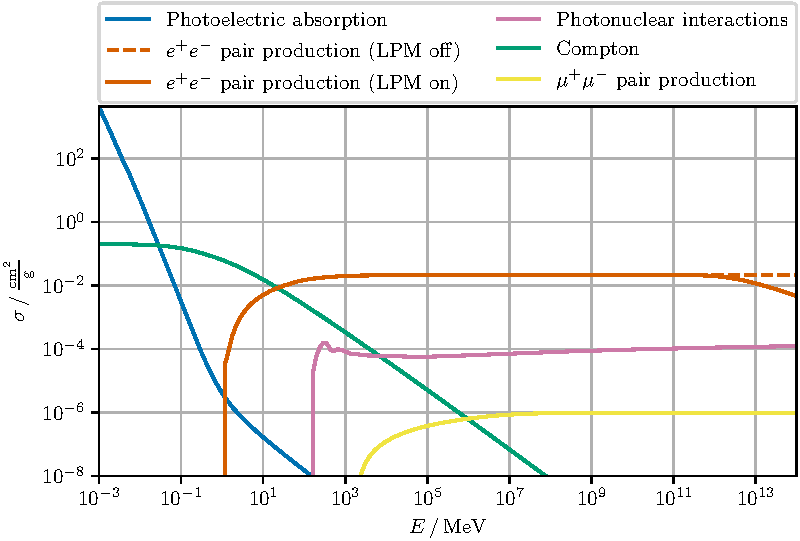
\includegraphics{../plots/Photon_Air_dndx_ecut_0.pdf}
    \caption{Total cross section of photons in air inside PROPOSAL.}
    \label{fig:total_cross_photon}
\end{figure}


\subsection{Photoelectric absorption}

Photoelectric absorption describes the ejection of an atomic electron due to its interaction with an in-going photon.
In this process, the photon energy is used to free the electron from its atomic binding, while the remaining photon energy serves as the kinetic energy of the now free electron.
For photons in air, photoelectric absorption becomes the dominant interaction process for energies below $\approx \SI{30}{\kilo\electronvolt}$.
In the context of electromagnetic cascades, photoelectric absorption as a process starts to become important for energies where its cross section represents a significant correction to the total mean free path length.

The detailed description of photoelectric absorption is non-trivial and dependent on the properties interaction target and its atomic structure.
Since the energy where photoelectric absorption becomes dominant is small, and the process is not important for the electromagnetic shower development, PROPOSAL only provides an approximate description based on the cross section given in \cite{heitler, sauter}.
The total cross section is defined as
%
\begin{align}
	\label{eqn:sauter}
	\sigma &= 4 \pi r_e^2 Z^5 \alpha^4 F_1 F_2 \left( \frac{m_e}{E} \right)^5 \left( \gamma^2 -1 \right)^{\sfrac{3}{2}} \left[ \frac{4}{3} + \frac{\gamma (\gamma - 2)}{\gamma + 1} \left( 1 - \frac{\ln{\left( \gamma + \sqrt{\gamma^2 - 1} \right)}}{\gamma \sqrt{\gamma^2 - 1}}  \right) \right],
\end{align}
%
with the photon energy $E$ and the definitions
\begin{align}
	\gamma &= 1 + \frac{E - I}{m_e}, & I &= \frac{Z^2 \alpha^2 m_e}{2}.
\end{align}
%
The term
\begin{align}
	F_1 &= \left[ 1 + \left( \frac{\alpha Z}{\beta} \right)^2 \right] \frac{\pi \alpha Z / \beta }{\sinh(\pi \alpha Z / \beta )} \exp\left[ \frac{\alpha Z}{\beta} \left( \pi - 4 \arctan\left( \frac{\beta}{\alpha Z} \right) \right) \right]
\end{align}
%
is used as a correction factor for the non-relativistic energy regime \cite{sauter}, while the term
%
\begin{align}
	F_2 &= 1 + 0.01481 \ln^2{Z} - 0.000788 \ln^3{Z}
\end{align}
%
is an empirical correction describing the ratio between the K-shell and total photoelectric absorption cross section \cite{hubbell1969}.

The photoelectric cross section and a validation of the total photon cross section at low energies is shown in Figure \ref{fig:photoeffect_nist}, where the total photon cross section in air is compared to the calculations from the NIST Standard Reference Database \cite{nist}.
Due to the approximative nature of the used photoelectric effect cross section, the deviations of up to \SI{10}{\percent} are expected.
For example, the K absorption line of argon at $E\approx\SI{3.2e-3}{\mega\electronvolt}$ is not well described by \eqref{eqn:sauter}.

\begin{figure}
	\centering
    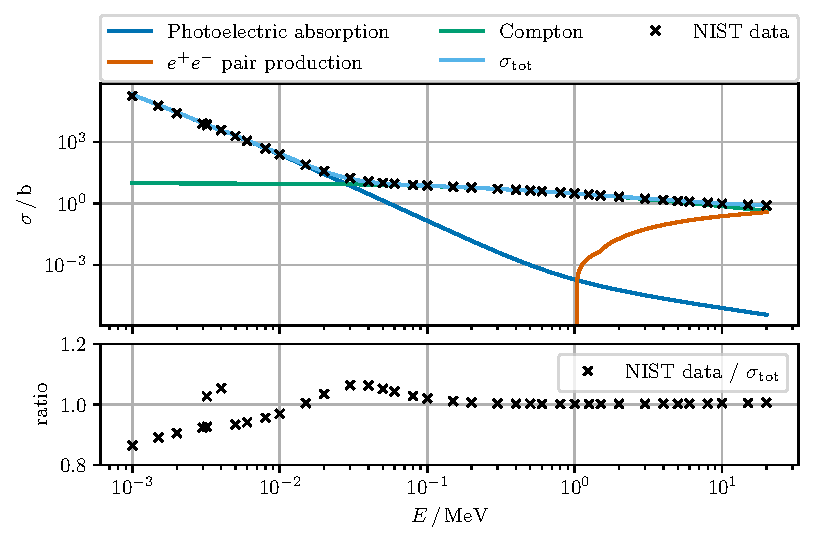
\includegraphics{../plots/photoeffect_nist.pdf}
    \caption{Photon cross sections in air for small energies, compared to the total cross section according to the NIST Standard Reference Database \cite{nist}.}
    \label{fig:photoeffect_nist}
\end{figure}

\subsection{Photonuclear interactions}

High-energy photons can perform hadronic interactions, in which the photon is absorbed by an atomic nucleus.
Although this process provides only a small contribution to the total mean free path length of photons for most energies, they are a source of hadronic particles, and consequently also muons from electromagnetic cascades.

In the context of nuclear muon interactions, parametrizations to describe photonuclear interactions of photons have already been implemented in PROPOSAL, but were only available internally.
These parametrization, which have been described in detail in \cite{KOEHNE20132070}, are now available to describe photonuclear interaction of real photons.

In addition, the parametrization from \cite{Heck2012CORSIKA}, which is also used in the simulation program CORSIKA~7, has also been implemented.
The continuous contribution of this cross section is given as 
%
\begin{align}
	\label{eqn:photonuclear_C7}
	\sigma_{\gamma,N} &=
	\begin{cases}
		\left(73.3 s^{0.073} + 191.7 s^{-0.602} \right) \sqrt{1 - s_0 / s} \si{\micro\barn}, & \text{for } \sqrt{s} \leq \SI{19.39}{\giga\electronvolt}, \\
		\left( 59.3 s^{0.093} + 120.2 s^{-0.358} \right) \si{\micro\barn}, & \text{for } \sqrt{s} > \SI{19.39}{\giga\electronvolt}, \\
	\end{cases}
\end{align} 
%
with $s = m_n^2 + 2 m_n E / \si{\giga\electronvolt}$ and the pion production threshold $\sqrt{s_0} = \SI{1.0761}{\giga\electronvolt}$.
In addition, the resonances for $\Delta(1232)$, $N(1520)$, and $N(1680)$ are superimposed on the continuous cross section, where the definition and parameters from \cite{Muecke_2000} are used.
Figure \ref{fig:photoproduction_cross} shows the different parametrizations for the photonuclear interactions implemented in PROPOSAL.
Note that both differences in the resonance region as well as in the extrapolation to high energies are visible.
%
\begin{figure}
	\centering
    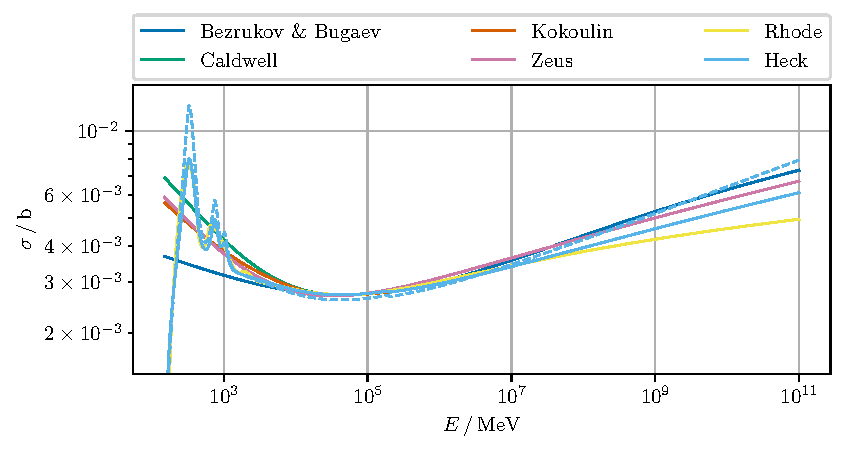
\includegraphics{../plots/photoproduction_cross.pdf}
    \caption{Photonuclear interaction cross sections implemented in PROPOSAL. For the Heck parametrization, the solid line indicates the shadowing parametrization according to \cite{KOEHNE20132070}, while for the dashed line, the shadowing parametrization $\sigma_{\gamma,A} = A^{0.91} \sigma_{\gamma,N}$ from \cite{Heck2012CORSIKA} has been used.}
    \label{fig:photoproduction_cross}
\end{figure}
%
Figure \ref{fig:total_cross_photon} shows the cross section of photonuclear interactions compared to other processes.
For energies where the LPM suppression of pair production becomes effective, the photonuclear process starts to become a significant contribution to the total photon cross section.

\subsection{Muon pair production}

Muon pair production describes the conversion of a photon to a muon pair in the field of an atomic nucleus.
While the contribution of this process to the mean free path length of photons is negligible compared to the dominant electron-positron pair production, it provides a source of muons from the electromagnetic shower component and therefore a potentially interesting event signature in extensive air showers.

Based on the muon bremsstrahlung cross section given in \cite{Kelner:288828}, the muon pair production cross section is given by
%
\begin{align}
	\begin{split}
		\frac{\mathrm{d}\sigma}{\mathrm{d}x} &= 4 Z^2 \alpha \left( r_e \frac{m_e}{m_\mu} \right)^2 \left[ 1 - \frac{4}{3} (x - x^2) \right] \\ &\times \Biggl( \Phi(\delta) + \frac{1}{Z} \left[ \ln\left( \frac{m_\mu / \delta}{\delta m_\mu / m_e^2 + \sqrt{e}} \right) - \ln\left( 1 + \frac{1}{\delta \sqrt{e} B^\prime Z^{\sfrac{-2}{3}} / m_e} \right) \right] \Biggr),
	\end{split}
\end{align}
%
where
%
\begin{align}
	\Phi(\delta) &= \underbrace{\ln \left( \frac{B Z^{\sfrac{-1}{3}} m_\mu / m_e}{1 + B Z^{\sfrac{-1}{3}} \sqrt{e} \delta / m_e } \right)}_{\Phi_0} - \underbrace{\ln\left( \frac{D_n}{1 + \delta (D_n \sqrt{e} - 2) / m_\mu} \right)}_{\Delta_\text{n}},
\end{align}
%
with the radiation logarithm constant $B$, the inelastic radiation logarithm $B^\prime$, and the definitions
%
\begin{align}
	x &= \frac{E_{\mu^-}}{E}, & \delta &= \frac{m_\mu^2}{2 E x (1 - x)}, & D_n &= 1.54 A^{0.27}.
\end{align}
%
For $Z > 1$, the effect of the inelastic nuclear form factor is included with the substitution
%
\begin{align}
	\Delta_\text{n} &\rightarrow \left( 1 - \frac{1}{Z} \right) \Delta_\text{n}.
\end{align}
%
The total cross section of muon pair production is shown in Figure \ref{fig:total_cross_photon}.

\subsection{Landau-Pomeranchuk-Migdal effect in electron-positron pair production}

The Landau-Pomeranchuk-Migdal effect is a suppression of bremsstrahlung and pair production processes occuring when the formation length reaches interatomic distances, which comes in effect for high energies and dense media.
The suppression is effective for small energy losses in case of bremsstrahlung, and for symmetric pair production events in case of electron-positron pair production.

Based on the parametrization of the LPM effect in \cite{RevModPhys.71.1501}, the suppression of the pair production cross section is given by
%
\begin{align}
	\label{eqn:lpm_photopair}
	\frac{\mathrm{d}\sigma_\text{LPM}}{\mathrm{d}x} &= \frac{\mathrm{d}\sigma}{\mathrm{d}x} \cdot \frac{\xi(s) / 3 \left(G(s) + 2 \left( x^2 + (1 - x)^2 \right) \phi(s) \right)}{1 - 4 / 3 x (1 - x)},
\end{align}
%
with $x = E_{e^{-}} / E$, where $E$ is the photon energy.
The functions $\xi(s)$, $G(s)$, $\phi(s)$, are given by \cite{PhysRevD.25.1291, PhysRev.103.1811}
%
\begin{align}
	\xi(s) &\approx \xi(s^\prime) =
	\begin{cases}
		2 & \text{if $s^\prime < s_1$}, \\
		1 + h - \frac{0.08 (1 - h) (1 - (1-h)^2)}{\ln{(s_1)}} & \text{if $s_1 \leq s^\prime < 1$}, \\
		1 & \text{if $s^\prime \geq 1$},
	\end{cases}
\end{align}
%
\begin{align}
	G(s) &=
	\begin{cases}
		3\psi(s) - 2\phi(s) & \text{if $s < \num{0.710390}$}, \\
		36s^2 / \left(36s^2 + 1 \right) & \text{if $\num{0.710390} \leq s < \num{0.904912}$}, \\
		1 - 0.022s^{-4} & \text{if $s \geq \num{0.904912}$},
	\end{cases}
\end{align}
%
\begin{align}
	\psi(s) &= 1 - \exp{\left\{ -4s - \frac{8s^2}{1 + 3.936s + 4.97s^2 - 0.05s^3 + 7.5 s^4} \right\}},
\end{align}
%
\begin{align}
	\phi(s) &=
	\begin{cases}
		1 - \exp{\left\{ -6s \left(1 + (3 - \pi) s\right) + \frac{s^3}{ 0.623 + 0.796s + 0.658 s^2} \right\}} & \text{if $s < \num{1.54954}$}, \\
		1 - 0.012 s^{-4} & \text{if $s \geq \num{1.54954}$},
	\end{cases}
\end{align}
%
with the variable definitions
%
\begin{align}
	s &= \frac{s^\prime}{\sqrt{\xi(s^\prime)}}, & s^\prime &= \frac{1}{8} \sqrt{\frac{E_\text{LPM}}{E x ( 1 - x)}}, & s_1 &= \frac{\sqrt{2} Z^{\sfrac{2}{3}}}{B^2}, \\ E_\text{LPM} &= \frac{2 \alpha (m_e c^2)^2 X_0}{\pi \hbar c}, & h &= \frac{\ln{(s^\prime)}}{\ln{(s_1)}}, & D_n &= 1.54 A^{0.27},
\end{align}
%
where $X_0$ is the radiation length and $B$ the radiation logarithm constant.

Figure \ref{fig:lpm_photopair_diff} shows the effect of the LPM suppression on the differential pair production cross section at different energies.
As expected, for $x = 0.5$, the suppression becomes maximal, while for $x \rightarrow 0$ and $x \rightarrow 1$, the suppression is zero.
Since the LPM effect depends on the material density, its suppression also depends on the height in the Earth's atmosphere.
In Figure \ref{fig:lpm_photopair_cross}, the suppression of the pair production cross section at different atmospheric heights is shown.
%
\begin{figure}
\centering
\begin{minipage}[t]{.48\textwidth}
  \centering
  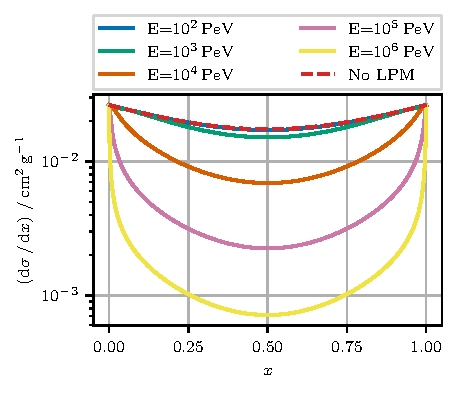
\includegraphics{../plots/lpm_photopair_differential_small.pdf}
  \captionof{figure}{Differential cross section for electron-positron pair production in air at sea level, with nitrogen as an interaction target. The effect of the LPM effect at different energies is shown. Note that without the LPM suppression, the differential cross section is almost identical for all energies in this plot.}
  \label{fig:lpm_photopair_diff}
\end{minipage}%
\hfill
\begin{minipage}[t]{.48\textwidth}
  \centering
  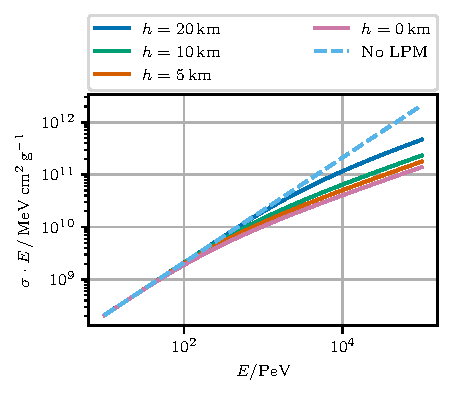
\includegraphics{../plots/lpm_cross_photopair_small.pdf}
  \captionof{figure}{Total cross section for electron-positron pair production in air, with the effect of the LPM suppression at different atmospheric heights.}
  \label{fig:lpm_photopair_cross}
\end{minipage}
\end{figure}